\documentclass[paper=a4,twoside=true,fontsize=11pt,numbers=noendperiod,chapterprefix=false]{scrbook}

%\usepackage[ngerman]{babel} %use this if you write you thesis in GERMAN!
%\usepackage[latin1]{inputenc}  %this is required if you want to use german umlauts in windows!
%\usepackage[applemac]{inputenc} % umlauts under Mac
%\usepackage[utf8]{inputenc} % umlauts if you have utf8 (recommended)

\usepackage{amsmath,amssymb,amsthm}
\usepackage[footnotesize,sl,SL,hang,tight]{subfigure}  
%\usepackage{float} %for positioning figures with H
\usepackage{longtable}
\usepackage[font={small,sl},hang,labelfont=bf]{caption} %italic,hanging,normalize   //margin=1cm
%\usepackage{captcont} % continue subfigures over several pages
\usepackage{booktabs}
%\usepackage{showkeys} % shows the labels above the references for easier development

% modify headings:
\usepackage{scrpage2}
\KOMAoptions{headinclude}

% Font packages:
\usepackage{times}
\usepackage{helvet}   % sets sans serif font
\usepackage[T1]{fontenc}

%PDF hyperref config
\ifpdfoutput{%
	\usepackage[pdftex]{graphicx}
	\usepackage[]{pdfpages} %for including full pdf pages
	\usepackage[pdftex,
		bookmarks,
		bookmarksopen=true,
		bookmarksnumbered=true,
		pdfauthor={My Name},
		pdftitle={Thesis Title},
		colorlinks,
		linkcolor=black,
		citecolor=black,
		filecolor=black,
		urlcolor=black,
		anchorcolor=black,
		menucolor=black,
		breaklinks=true,
		pageanchor=true, %for jumping to a page
		plainpages=false,
		pdfpagelabels=true]{hyperref}
	\pdfcompresslevel=9
	\pdfoutput=1
	\pdfminorversion=6
	\DeclareGraphicsExtensions{.pdf,.png}
}{
	\usepackage{graphicx}
}
\usepackage{rotating} % rotate figures, must be loaded after graphicx!

\usepackage[printonlyused]{acronym} % Abbreviations list

\bibliographystyle{alpha}

% Uncomment the chapter / section you are working on.
%
%\includeonly{chapter}
%\pagestyle{useheadings}

% A4 page layout
% A4 = 210 x 297 mm /	 1in = 25.4mm / margin becomes margin + 1in in latex!
\topmargin -12.7mm
\textheight 234.0mm
\textwidth 160.0mm
\oddsidemargin 4.57mm
\evensidemargin -5.59mm
\parskip 2.54mm
\parindent 0mm
\headsep 15mm
%\footskip 10mm

\renewcommand{\arraystretch}{1.5}
\renewcommand{\baselinestretch}{1}

\input{preamble}

\begin{document}

%% Define leading chapter pages
%
\input{studchapter}
\newpagestyle{mychapterpagestyle}{{\protect\mychpstyleintl}{\protect\mychpstyleintl}}{}
\newpagestyle{myappendixpagestyle}{{\protect\mychpstyleintl}{\protect\mychpstyleintl}}{}
%%

%% macros
\newcommand{\mykeyword}[0]{my long text}
%reference macros -> change this if you write you thesis in an other language!!!
\newcommand{\chpref}[1]{Chapter \ref{#1}}
\newcommand{\secref}[1]{Section \ref{#1}}
%\newcommand{\equref}[1]{Equation \ref{#1}} %better use builtin \eqref{} !!!
\newcommand{\figref}[1]{Figure \ref{#1}}
\newcommand{\tabref}[1]{Table \ref{#1}}
\newcommand{\apxref}[1]{Appendix \ref{#1}}
%%

%---------------
%% Title page:
%---------------
\pagenumbering{arabic} %pagenumbering for title
\setcounter{page}{-1}  %required in order not to have more pages with pagenumber 1
%\title{Book Title}
%\author{My Name}
%\date{January 2007}
%\maketitle
%\clearemptydoublepage
% --- selfmade version ----
\begin{titlepage}
	\topmargin -3.8cm
	\oddsidemargin 0.0cm
	\evensidemargin 0.0cm
	\centering
%	\begin{minipage}{0.49\textwidth}
%		\vspace{0pt}
%		\includegraphics*[width=0.8\textwidth]{figures/title/ETH_logo}
%		\vfill
%	\end{minipage}
%	\begin{minipage}{0.49\textwidth}
%		\vspace{0pt}
%		\hfill
%		\includegraphics*[width=0.6\textwidth]{figures/title/logo_inspire_icvr}
%	\end{minipage}
%	\\
	\includegraphics*[width=0.38\textwidth]{figures/title/ETH_logo} \hfill
	% Choose your logo here!
	\includegraphics*[width=0.21\textwidth]{figures/title/loco_icvr} \\
	%\includegraphics*[width=0.21\textwidth]{figures/title/logo_inspire_ics} \\
	%\includegraphics*[width=0.24\textwidth]{figures/title/logo_inspire_icvr} \\
	%\includegraphics*[width=0.24\textwidth]{figures/title/logo_inspire_irpd} \\
	\vspace{8.2cm}
	\Huge
	\textbf{\textsf{Thesis Title}} \\[2.0cm]
	%\includegraphics*[width=0.4\textwidth]{figures/title/mytitlefigure} 
	\vspace{5.0cm}
	\sffamily
	\Large
	My Name
	\\[0.8cm]
	\large
	Master Thesis or Bachelor Thesis
	\\
	Date
	\\[0.8cm] %anstatt 1.5cm
	Supervisor Name
	\\[0.5cm]
	Prof. Name
	\vfill
\end{titlepage}
\clearemptydoublepage
%%

\pagenumbering{roman}
\setcounter{page}{1}

\chapter*{Abstract}
%Context, Content and Conclusion summarized to 1 page.
% English version:

Experimental modal analysis in tandem with the modal model of a machine tool is a powerful tool for the evaluation of the machine tools' dynamic behavior. But because experimental modal analysis is an expensive procedure, both due to high instrument costs and the need for experienced operators, the modal model is often not verified.

With the aim to decrease instrument costs and increase the use of experimental modal analysis, the system presented in this thesis consists of a micro controller based data acquisition system, a modal impact hammer and a low-cost accelerometer. The latter is a capacitive micro-electro-mechanical-sensor and the impact hammer is using a strain gauge load cell as impact sensor.

For the implementation of a low-cost modal analysis system based on the aforementioned components a micro controller based bus system and a specialized communication protocol is suggested.

%------------------------------------------
\cleardoublepage{}
\chapter*{Zusammenfassung}

Die experimentelle Modalanalyse, in Kombination mit dem modalen Modell einer Werkzeugmaschine, ist ein mächtiges Werkzeug, um das dynamische Verhalten der Werkzeugmaschine zu evaluieren. Teure Messinstrumente und der Bedarf an erfahrenen Bedienern machen die experimentelle Modalanalyse allerdings zu einem kostspieligen Unterfangen. Oft wird daher das modale Modell gar nicht validiert.

Mit dem Ziel die Kosten für Messinstrumente zu senken und den Gebrauch von experimenteller Modalanalyse zu steigern, wird in dieser Arbeit ein System vorgestellt, welches aus einem Mikrokontroller-basierten Datenakquisitionssystem, einem Impulshammer und einem kostengünstigen Beschleunigungssensor besteht. Letzterer ist ein kapazitiver mikro-elektro-mechanischer Senor und der Impulshammer ist mit einer Dehnmessstreifen basierten Ladungszelle ausgestattet.

Für die Umsetzung eines kostengünstigen Modalanalysesystems auf der Grundlage der zuvor genannten Komponenten, wird ein Mikrokontroller-basiertes Bus-System mit einem spezialisierten Kommunikationsprotokoll vorgeschlagen.


%task description
\cleardoublepage
%\includegraphics[viewport=3cm 0cm 20cm 27.5cm]{task_description}
\includepdf{task_description.pdf}
\cleardoublepage

\chapter*{Acknowledgment}

I would like to thank Natanael Lanz for his aid in sensor characteristics, Daniel Spescha for his inputs on modal analysis and Nino Ceresa for his continued support while all was happening from remote locations during this unusual year.


\tableofcontents
\cleardoublepage

\listoffigures
\addcontentsline{toc}{chapter}{List of Figures}
\cleardoublepage

\listoftables
\addcontentsline{toc}{chapter}{List of Tables}
\cleardoublepage


\addcontentsline{toc}{chapter}{List of Abbreviations} 
\chapter*{List of Abbreviations}

\begin{acronym}[ESEVNEI] % Put the longest abbreviation in the square brackets for proper alignment
 \acro{CCCED}{Ceterum censeo Carthaginem esse delendam}
 \acro{SQL}{Structured Query Language}
 \acro{EBNEV}{Extra Bavariam Non Est Vita}
 \acro{ESEVNEI}{Et Si Est Vita Non Est Ita}
 \acro{VM}{Virtuelle Maschine}
\end{acronym}
\cleardoublepage

\addcontentsline{toc}{chapter}{List of Symbols} 
\chapter*{List of Symbols}

\begin{center}

	\begin{tabular}{lll} \hline
		Symbol & Unit & Description\\ \hline
		$\alpha$ & $^{\circ}$ & General angle \\
		$F_{N, Eff.}$ & $N$ & Effective Normal Force acting upon the center of gravity \\
	\end{tabular}

\end{center}
\cleardoublepage

\pagenumbering{arabic}
\renewcommand*{\chapterpagestyle}{mychapterpagestyle}
\renewcommand*{\chapterformat}{} % show chapter titles only (no numbers)
% \setchapterpreamble[o]{...}  unfortunately does not move the \chapter output downwards


% ---- MAIN PART ----
% set counter to n-1:
\setcounter{chapter}{0}

\chapter{Introduction}

%-----------------------------------------------------
\section{Motivation}
The \ac{EMA} is a powerful tool for evaluating dynamic models of structures. Despite its extensive usage in the aerospace industry, in many other engineering fields the benefits of \ac{EMA} are overshadowed by the initial investment and the operator costs of an \ac{EMA} system. To enable \ac{MT} manufactures to test their products and validate their modal predictions. Progress in \ac{MEMS} technology enables the use of new generation of low-cost senors in \ac{EMA}.

%-----------------------------------------------------
\section{Related Work}

Considering the use of low-cost accelerometers in \ac{EMA} specifically, a two-point vibration measurement system with a bandwidth of \SI{500}{\hertz} has been developed \cite{chan2017multiple}. The authors \citeauthor{chan2017multiple} used this system to conduct a multiple-point vibration test a \ac{MT}. Operating at lower frequencies, \citeauthor{beskhyroun2012low} used \ac{MEMS} based accelerometers to conduct an \ac{EMA} on building structures. \citeauthor{piana2016experimental} developed a modal test system, which uses piezoelectric transducers that are typically used to tune musical instruments as response sensors \cite{piana2016experimental}. Moreover, a construction kit for a low-cost vibration analysis system was proposed by \citeauthor{vollmer2009construction} back in 2009 \cite{vollmer2009construction}.

In the field of civil engineering, bridges and skyscrapers require continuous vibration signal logging for structural health monitoring. This leads to an increased interest in driving down the cost of accelerometer based vibration monitoring systems. \citeauthor{girolami2018modal} has developed a low-cost \ac{MEMS} systems for structural health monitoring of civil structures \cite{girolami2018modal}.

Structural health monitoring is also required in rotary systems such as gas and wind turbines. \citeauthor{esu2014integration} integrated low-cost accelerometers in wind turbines and logged data via radio frequency to a central device.

Addressing low-cost impact hammer constructions, \citeauthor{waltham2009construction} implemented a piezoelectric transducer in a hammer, that is designed to trigger barbecue lighters \cite{waltham2009construction}. And for inexpensive calibration of a load cell used for modal testing, \citeauthor{wang2015practical} introduced practical techniques \cite{wang2015practical}.

%-----------------------------------------------------
\section{Overview}

First fundamentals in measurement instrumentation, sensors and \ac{EMA} is introduced in the state of the art. Then the \acf{DAC} developed for this project is presented in \autoref{chap:dac_software}. Testing environment are described in the \autoref{chap:test_setups} and measurement results are discussed in results. Finally the conclusion gives reflects on the project.


% add your chapter files here!
\chapter{Sample Chapter}
\label{chp:sample_chapter}
In this chapter we present the main part of the bla bla.

%***********************************************************************
\section{Formula Use Example}
\label{sec:forumla}
Lorem ipsum dolor sit amet, consectetuer adipiscing elit, sed diam nonummy nibh euismod tincidunt ut laoreet dolore magna aliquam erat volutpat. \ac{EBNEV}, \ac{ESEVNEI}. \ac{CCCED}. Ut wisi enim ad minim veniam, quis nostrud exerci tation ullamcorper suscipit lobortis nisl ut aliquip ex ea commodo consequat \ac{SQL}. 

To calculate the mean of n values $\mathbf{x} = [x_1, x_2, ..., x_n]$, we use
\begin{equation}
	\bar{x} = \frac{1}{n} \sum_{i=1}^{n}{x_i}
	\label{eq:emp_mean}
\end{equation}


\subsection{Sample Subsection with References}
\label{sec:sample_subsection}
An equation in inline style looks like this $p(w_j)$.

Here we give examples how to create references:
\begin{itemize}
% Note that you can only reference to labels (except for citations).
% The way how you name your labels is up to you! The style "\label{type:name}" in this template is only a suggestion.
	\item a chapter reference: \chpref{chp:sample_chapter}
	\item a section reference: \secref{sec:sample_section}
	\item an equation reference: \eqref{eq:emp_mean}
	\item a figure reference: \figref{fig:sample1}
	\item a table reference: \tabref{tab:longlist} in \apxref{apx:appendix}
	\item a citation if BibTex is used: \cite{Iwata07}
	\item mutiple citations: \cite{Su07,Feasel08}
\end{itemize}


%***********************************************************************
\section{Sample Section with Figures}
\label{sec:sample_section}
Lorem ipsum dolor sit amet, consectetuer adipiscing elit, sed diam nonummy nibh euismod tincidunt ut laoreet dolore magna aliquam erat volutpat. Ut wisi enim ad minim veniam, quis nostrud exerci tation ullamcorper suscipit lobortis nisl ut aliquip ex ea commodo consequat. Duis autem vel eum iriure dolor in hendrerit in vulputate velit esse molestie consequat, vel illum dolore eu feugiat nulla facilisis at vero et accumsan et iusto odio dignissim qui blandit praesent luptatum zzril delenit augue duis dolore te feugait nulla facilisi. Lorem ipsum dolor sit amet, consectetuer adipiscing elit, sed diam nonummy nibh euismod tincidunt ut laoreet dolore magna aliquam erat volutpat. Ut wisi enim ad minim veniam, quis nostrud exerci tation ullamcorper suscipit lobortis nisl ut aliquip ex ea commodo consequat. Duis autem vel eum iriure dolor in hendrerit in vulputate velit esse molestie consequat, vel illum dolore eu feugiat nulla facilisis at vero et accumsan et iusto odio dignissim qui blandit praesent luptatum zzril delenit augue duis dolore te feugait nulla facilisi. Nam liber tempor cum soluta nobis eleifend option congue nihil imperdiet doming id quod mazim placerat facer possim assum. See \figref{fig:sample1}.

\begin{figure}[!htb]
    \centering
    \includegraphics[width=0.8\linewidth]{figures/samples/sample1} %NOTE that no .pdf has to be written
    \caption[Some other short caption]{Lorem ipsum dolor sit amet, consectetuer adipiscing elit, sed diam nonummy nibh euismod tincidunt ut laoreet dolore magna aliquam erat volutpat. Ut wisi enim ad minim veniam, quis nostrud exerci tation ullamcorper suscipit lobortis nisl ut aliquip ex ea commodo consequat. Duis autem vel eum iriure dolor in hendrerit in vulputate velit esse molestie consequat, vel illum dolore eu feugiat nulla facilisis at vero et accumsan et iusto odio dignissim qui blandit praesent luptatum zzril delenit augue duis dolore te feugait nulla facilisi. Lorem ipsum dolor sit amet, consectetuer adipiscing elit, sed diam nonummy nibh euismod.}
    \label{fig:sample1}
\end{figure}



%-------------------------------
\subsection{Subfigure Use Example}
Ipsum dolor sit amet, consectetuer adipiscing elit, sed diam nonummy nibh euismod tincidunt ut laoreet dolore magna aliquam erat volutpat. Ut wisi enim ad minim veniam, quis nostrud exerci tation ullamcorper suscipit lobortis nisl ut aliquip ex ea commodo consequat.
\begin{figure}[!htb]
	\centering
	\subfigure[Caption 1]{\label{fig:sf1}\includegraphics[width=0.4\textwidth]{figures/title/ETH_logo}} \hfill
	\subfigure[Caption 2]{\label{fig:sf2}\includegraphics[width=0.4\textwidth]{figures/title/ETH_logo}}
	\subfigure[Caption 3]{\label{fig:sf3}\includegraphics[width=0.4\textwidth]{figures/title/ETH_logo}} \hfill
	\subfigure[Caption 4]{\label{fig:sf4}\includegraphics[width=0.4\textwidth]{figures/title/ETH_logo}}
	\caption[Short Caption]{Long caption. Lorem ipsum dolor sit amet, consectetuer adipiscing elit, sed diam nonummy nibh euismod tincidunt ut laoreet dolore magna aliquam erat volutpat. Ut wisi enim ad minim veniam, quis nostrud exerci tation ullamcorper suscipit lobortis nisl ut aliquip ex ea commodo consequat. Figure subreference inside a caption: \subref{fig:sf4}.}
	\label{fig:sf_sample}
\end{figure}

Subfigure reference: \figref{fig:sf2}.

%-------------------------------
\subsection{Further Table and Figure Examples}
\label{sec:impr_wd}
Lorem ipsum dolor sit amet, consectetuer adipiscing elit, sed diam nonummy nibh euismod tincidunt ut laoreet dolore magna aliquam erat volutpat. Ut wisi enim ad minim veniam, quis nostrud exerci tation ullamcorper suscipit lobortis nisl ut aliquip ex ea commodo consequat. Duis autem vel eum iriure dolor in hendrerit in vulputate velit esse molestie consequat, vel illum dolore eu feugiat nulla facilisis at vero et accumsan et iusto odio dignissim qui blandit praesent luptatum zzril delenit augue duis dolore te feugait nulla facilisi. Lorem ipsum dolor sit amet, consectetuer adipiscing elit, sed diam nonummy nibh euismod tincidunt ut laoreet dolore magna aliquam erat volutpat. Ut wisi enim ad minim veniam, quis nostrud exerci tation ullamcorper suscipit lobortis nisl ut aliquip ex ea commodo consequat. See \tabref{tab:imprwdpatterns}.
\begin{table}[!htb]
	\footnotesize
	\centering
		\begin{tabular}{cll}
			\toprule
			Number & Something & Something Else \\
			\midrule
			1 & Blup & 1 | 2 | 3 | 4 | 5 | 6 | 7 \\
			2 & Blup & 1 | 2 | 3 | 4 | 5 | 6 | \emph{blip} \\
			3 & Blup & 1 | 2 | 3 | 4 | 5 | 6 | 7 \\
			4 & Blup & 1 | 2 | 3 | 4 | 5 | 6 \\
			5 & Blup & that's it \\
			\bottomrule
		\end{tabular}
	\normalsize
	\caption[Short caption]{Lorem ipsum dolor sit amet, consectetuer adipiscing elit, sed diam nonummy nibh euismod tincidunt ut laoreet dolore magna aliquam erat volutpat. Ut wisi enim ad minim veniam, quis nostrud exerci tation ullamcorper suscipit lobortis nisl ut aliquip ex ea commodo consequat.}
	\label{tab:imprwdpatterns}
\end{table}

Lorem ipsum dolor sit amet, consectetuer adipiscing elit, sed diam nonummy nibh euismod tincidunt ut laoreet dolore magna aliquam erat volutpat. Ut wisi enim ad minim veniam, quis nostrud exerci tation ullamcorper suscipit lobortis nisl ut aliquip ex ea commodo consequat.

\begin{table}[!htb]
	\begin{minipage}{0.45\textwidth}
		\centering
		\footnotesize
		\begin{tabular}{lrr}
			 \hline
    	 \textbf{First} & \textbf{Second} & \textbf{Third} \\
    	 \hline
			Table & -0.20  & 4.5E-2 \\
			Table & 0.07 & 6.6E-2 \\
			Table & 0.06 & 2.0E-1 \\
			Table & 0.20 & 1.8E-5 \\
			Table & 0.38 & 1.3E-4 \\
			Table & 0.32 & 9.5E-5 \\
			Table & 0.49 & 6.9E-8 \\
			\hline
  	\end{tabular}
  	\normalsize
	\end{minipage} \hfill
	\begin{minipage}{0.54\textwidth}
		\centering
		\includegraphics[width=0.5\linewidth]{figures/samples/sample2}
	\end{minipage}
	\caption[Some short caption]{Lorem ipsum dolor sit amet, consectetuer adipiscing elit, sed diam nonummy nibh euismod tincidunt ut laoreet dolore magna aliquam erat volutpat. Ut wisi enim ad minim veniam, quis nostrud exerci tation ullamcorper suscipit lobortis nisl ut aliquip ex ea commodo consequat.}
	\label{tab:imprwd_params}
\end{table}


Ipsum dolor sit amet, consectetuer adipiscing elit, sed diam nonummy nibh euismod tincidunt ut laoreet dolore magna aliquam erat volutpat. Ut wisi enim ad minim veniam, quis nostrud exerci tation ullamcorper suscipit lobortis nisl ut aliquip ex ea commodo consequat. Duis autem vel eum iriure dolor in hendrerit in vulputate velit esse molestie consequat, vel illum dolore eu feugiat nulla facilisis at vero et accumsan et iusto odio dignissim qui blandit praesent luptatum zzril delenit augue duis dolore te feugait nulla facilisi. Lorem ipsum dolor sit amet, consectetuer adipiscing elit, sed diam nonummy nibh euismod tincidunt ut laoreet dolore magna aliquam erat volutpat. Ut wisi enim ad minim veniam, quis nostrud exerci tation ullamcorper suscipit lobortis nisl ut aliquip ex ea commodo consequat. Duis autem vel eum iriure dolor in hendrerit in vulputate velit esse molestie consequat, vel illum dolore eu feugiat nulla facilisis at vero et accumsan et iusto odio dignissim qui blandit praesent luptatum zzril delenit augue duis dolore te feugait nulla facilisi. Nam liber tempor cum soluta nobis eleifend option congue nihil imperdiet doming id quod mazim placerat facer possim assum.




\chapter{Results and Discussion}
\label{chap:results}

In this chapter excerpt of the results using the above setups is presented.

%***********************************
\section{Hammer-Hammer Test}

The results of the hammer-hammer test are impulse signal recordings of both, the reference system and the prototype \ac{LC}. Because the prototype signal is not calibrated, in order to able to compare the signals one needs to normalize the signal range of the reference signal. Furthermore, the signals need to be synced in time, by applying a time shift to one. The outputs gained after these transformations are shown in \figref{fig:HH_comparison}.

It can be seen that if one is using the soft PVC tip of the reference system both signals correlate well. If we then focus on the detailed view of such a test, as seen in \figref{fig:HH_noise}, the difference in resolution becomes apparent.

\begin{figure}[!htb]
  \centering
  \includestandalone[width=0.9\linewidth]{figures/test_setups/HH_comparison/HH_comparison}
  \caption[HH-Test comparison]{The HH-Test recordings of the reference hammer (orange) and the evaluated impact hammer system (turquoise). Note that the evaluated signal values are normalized so that the maxima are equal to the reference system.%
    \label{fig:HH_comparison}}
\end{figure}
\begin{figure}[!htb]
  \centering
  \includestandalone[width=\linewidth]{figures/test_setups/HH_noise/HH_noise}
  \caption[HH006 Plot]{Detailed plot of HH-Test 006%
    \label{fig:HH_noise}}
\end{figure}

\section{Andromeda Measurement}
Before comparing the accelerometer signals of the reference with the ones of the prototype system, one needs to subtract the constant gravitational part from the prototype signals. Additionally, the signals need to be synchronized in the time axis, as can be seen in \figref{fig:HAp024_TDat_z}.

When we then consider the frequency domain of \figref{fig:HAp024_FFTa_z} one can see that both signals cover the excited frequency bandwidth of around \SI{250}{\hertz} in a similar manner. The initial deviation at \SI{1}{\hertz} can be explained due to the signal conditioning in the reference system, where lower frequencies are cut-off.

\begin{figure}[!htb]
  \centering
  \includestandalone[width=0.95\linewidth]{figures/results/HAp024_TDat_z}
  \caption[Andromeda Measurement HAp024, Time Domain in Z-Axis]{Measurement HAp024 in the time domain, excitation at point A, as shown in \figref{fig:andromeda_positions}%
    \label{fig:HAp024_TDat_z}}
\end{figure}
\begin{figure}[!htb]
  \centering
  \includestandalone[width=0.95\linewidth]{figures/results/HAp024_FFTa_z}
  \caption[Andromeda Measurement HAp024, FFT in Z-Axis]{Measurement FFT HAp024, excitation at point A, as shown in \figref{fig:andromeda_positions}%
    \label{fig:HAp024_FFTa_z}}
\end{figure}
\clearpage

\section{Filter Test Setups}
The implementation of \figref{sfig:dac_comp_precond} is an iteration on the setup without a filter. But for the verification of the filter function a test setup was needed. But because of incompatibilities between the variable clock generator and the clock tunable filters, no meaningful output signals could be measured.

\chapter{Conclusion and Future Work}

%***********************************************************************
\section{Conclusion}
In this thesis
\begin{itemize}
  \item A low-cost capacitive accelerometer \ac{IC} has been used to measure the output signal of an \ac{EMA} measurement setup
  \item An impulse hammer using a strain gauge load cell has been developed using low-cost components.
  \item Different conditioning filter circuits have been studied for the impulse hammer signal
  \item A data packaging and communication protocol has been developed
\end{itemize}

\subsection{Deficiencies}
Because of the lack of a thorough state of the art research in the beginning of the project, the solution space of the project has been constricted early on. In this solution space, the data rates and the required compute efficiency of \ac{MCU}s were not met by the software. Furthermore, the issue of conditioning the analog signal of the \ac{LC} signal has been addressed at a late stage. Leading to no successful hardware setup with an upstream \ac{LPF}.

\newpage
%***********************************************************************
\section{Future Work}
There are multiple options to progress from this point. They can be framed in ... directions:
\begin{itemize}
  \item Explore the same solution space further, i.e.\ handling the \ac{LPF} circuit and optimizing the software.
  \item Change to a different solution space with either standard components using \ac{CPU}s or \ac{FPGA}s, targeting simpler implementation or higher bandwidths
  \item Exploring the limits of the application and limits current solution without additional preconditioning
\end{itemize}

Independent of the chosen direction one can progress by
\begin{itemize}
  \item Testing the limits of multi channelling
  \item Leaving the prototyping stage and simplify the production
  \item Exploring wireless communication
\end{itemize}



\appendix
\clearpage
\renewcommand*{\chapterpagestyle}{myappendixpagestyle}
\chapter{Appendix}
\label{apx:appendix}

{\scriptsize%
\begin{longtable}{lccc}
\caption[Andromeda Measurements, Prototype Impact Hammer]{Andromeda measurement setup that is excited by the prototype impact hammer. The prototype accelerometer is set to a dynamic range of $\pm$\SI{16}{g} and a \acs{AAF} cut-off of \SI{800}{\hertz}.}\\
\toprule
Label & \makecell{Excitation\\Location} & \makecell{Prototype Sampling\\Rate / \si{\kilo\hertz}} & \makecell{Prototype Recording\\Duration / \si{\second}}\\
\midrule
\endfirsthead
\caption[]{(Continued)}\\
\toprule
Label & \makecell{Excitation\\Location} & \makecell{Prototype Sampling\\Rate / \si{\kilo\hertz}} & \makecell{Prototype Recording\\Duration / \si{\second}}\\
\midrule
\endhead
\midrule
\multicolumn{4}{c}{continued on next page}\\
\bottomrule
\endfoot
%\bottomrule
\endlastfoot
\hline
	HAe001 & A & 1.6 & 3\\ 
	HAe002 & A & 1.6 & 3\\ 
	HAe003 & A & 1.6 & 3\\ 
	HAe004 & A & 1.6 & 3\\ 
	HAe005 & A & 1.6 & 3\\ 
	HAe006 & B & 1.6 & 3\\
	HAe007 & B & 1.6 & 3\\
	HAe008 & B & 1.6 & 3\\
	HAe009 & B & 1.6 & 3\\
	HAe010 & B & 1.6 & 3\\
	HAe011 & C & 1.6 & 3\\
	HAe012 & C & 1.6 & 3\\
	HAe013 & C & 1.6 & 3\\
	HAe014 & C & 1.6 & 3\\
	HAe015 & C & 1.6 & 3\\
	HAe016 & D & 1.6 & 3\\
	HAe017 & D & 1.6 & 3\\
	HAe018 & D & 1.6 & 3\\
	HAe019 & D & 1.6 & 3\\
	HAe020 & D & 1.6 & 3\\
\bottomrule
\label{tab:hae_tests}
\end{longtable}
}

{\scriptsize%
\begin{longtable}{lccccc}
\caption[Andromeda Measurements, Reference Impact Hammer]{Andromeda measurement setup that is excited by the reference impact hammer}\\
\toprule
Label & \makecell{Excitation\\Location} & \makecell{Accelerometer Sampling\\Rate / \si{\kilo\hertz}} & \makecell{Prototype Recording\\Duration / \si{\second}} & \makecell{Accelrometer\\Dynamic Range / \si{g}} & \makecell{Accelerometer\\AAF cut-off / \si{\hertz}}\\
\midrule
\endfirsthead
\caption[]{(Continued)}\\
\toprule
Label & \makecell{Excitation\\Location} & \makecell{Accelerometer Sampling\\Rate / \si{\kilo\hertz}} & \makecell{Prototype Recording\\Duration / \si{\second}} & \makecell{Accelrometer\\Dynamic Range / \si{g}} & \makecell{Accelerometer\\AAF cut-off / \si{\hertz}}\\
\midrule
\endhead
\midrule
\multicolumn{6}{c}{continued on next page}\\
\bottomrule
\endfoot
%\bottomrule
\endlastfoot
\hline
    HAp001 & A & 1.6 & 3 & $\pm$16 & 800\\
	HAp002 & A & 1.6 & 3 & $\pm$16 & 800\\
	HAp003 & A & 1.6 & 3 & $\pm$16 & 800\\
	HAp004 & A & 1.6 & 3 & $\pm$16 & 800\\
	HAp005 & A & 1.6 & 3 & $\pm$16 & 800\\
	HAp006 & B & 1.6 & 3 & $\pm$16 & 800\\
	HAp007 & B & 1.6 & 3 & $\pm$16 & 800\\
	HAp008 & B & 1.6 & 3 & $\pm$16 & 800\\
	HAp009 & B & 1.6 & 3 & $\pm$16 & 800\\
	HAp010 & B & 1.6 & 3 & $\pm$16 & 800\\
	HAp011 & C & 1.6 & 3 & $\pm$16 & 800\\
	HAp012 & C & 1.6 & 3 & $\pm$16 & 800\\
	HAp013 & C & 1.6 & 3 & $\pm$16 & 800\\
	HAp014 & C & 1.6 & 3 & $\pm$16 & 800\\
	HAp015 & C & 1.6 & 3 & $\pm$16 & 800\\
	HAp016 & D & 1.6 & 3 & $\pm$16 & 800\\
	HAp017 & D & 1.6 & 3 & $\pm$16 & 800\\
	HAp018 & D & 1.6 & 3 & $\pm$16 & 800\\
	HAp019 & D & 1.6 & 3 & $\pm$16 & 800\\
	HAp020 & D & 1.6 & 3 & $\pm$16 & 800\\
	HAp001 & A & 0.8 & 3 & $\pm$16 & 400\\
	HAp002 & A & 0.8 & 3 & $\pm$16 & 400\\
	HAp003 & A & 0.8 & 3 & $\pm$16 & 400\\
	HAp004 & A & 0.8 & 3 & $\pm$16 & 400\\
	HAp005 & A & 0.8 & 3 & $\pm$16 & 400\\
	HAp006 & B & 0.8 & 3 & $\pm$16 & 400\\
	HAp007 & B & 0.8 & 3 & $\pm$16 & 400\\
	HAp008 & B & 0.8 & 3 & $\pm$16 & 400\\
	HAp009 & B & 0.8 & 3 & $\pm$16 & 400\\
	HAp010 & B & 0.8 & 3 & $\pm$16 & 400\\
	HAp011 & C & 0.8 & 3 & $\pm$16 & 400\\
	HAp012 & C & 0.8 & 3 & $\pm$16 & 400\\
	HAp013 & C & 0.8 & 3 & $\pm$16 & 400\\
	HAp014 & C & 0.8 & 3 & $\pm$16 & 400\\
	HAp015 & C & 0.8 & 3 & $\pm$16 & 400\\
	HAp016 & D & 0.8 & 3 & $\pm$16 & 400\\
	HAp017 & D & 0.8 & 3 & $\pm$16 & 400\\
	HAp018 & D & 0.8 & 3 & $\pm$16 & 400\\
	HAp019 & D & 0.8 & 3 & $\pm$16 & 400\\
	HAp020 & D & 0.8 & 3 & $\pm$16 & 400\\
	HAp021 & C & 1.6 & 3 & $\pm$4 & 800\\
	HAp022 & C & 1.6 & 3 & $\pm$4 & 800\\
	HAp023 & C & 1.6 & 3 & $\pm$4 & 800\\
	HAp024 & C & 1.6 & 3 & $\pm$4 & 800\\
	HAp025 & C & 1.6 & 3 & $\pm$4 & 800\\
	HAp026 & D & 1.6 & 3 & $\pm$2 & 800\\
	HAp027 & D & 1.6 & 3 & $\pm$2 & 800\\
	HAp028 & D & 1.6 & 3 & $\pm$4 & 800\\
	HAp029 & D & 1.6 & 3 & $\pm$4 & 800\\
	HAp030 & D & 1.6 & 3 & $\pm$4 & 800\\
\bottomrule
\label{tab:hap_tests}
\end{longtable}
}

{\scriptsize%
\begin{longtable}{lccc}
\caption[Hammer-Hammer Test Measurements]{Hammer-hammer test measurements}\\
\toprule
Label & \makecell{Prototype\\tip} & \makecell{Prototype Sampling\\Rate / \si{\kilo\hertz}} & \makecell{Prototype Recording\\Duration / \si{\second}}\\
\midrule
\endfirsthead
\caption[]{(Continued)}\\
\toprule
Label & \makecell{Prototype\\tip} & \makecell{Prototype Sampling\\Rate / \si{\kilo\hertz}} & \makecell{Prototype Recording\\Duration / \si{\second}}\\
\midrule
\endhead
\midrule
\multicolumn{4}{c}{continued on next page}\\
\bottomrule
\endfoot
%\bottomrule
\endlastfoot
\hline
	HH001 & 34CrMo4 & 3 & 4\\
	HH002 & 34CrMo4 & 3 & 4\\
	HH003 & 34CrMo4 & 3 & 4\\
	HH004 & 34CrMo4 & 3 & 4\\
	HH005 & 34CrMo4 & 3 & 4\\
	HH006 & 34CrMo4 & 3 & 4\\
	HH007 & 34CrMo4 & 3 & 4\\
	HH008 & 34CrMo4 & 3 & 4\\
	HH009 & 34CrMo4 & 3 & 4\\
	HH010 & 34CrMo4 & 3 & 4\\
	HH011 & 34CrMo4 & 3 & 3\\
	HH012 & 34CrMo4 & 2 & 3\\
	HH013 & 34CrMo4 & 2 & 3\\
	HH014 & 34CrMo4 & 2 & 3\\
	HH015 & 34CrMo4 & 2 & 3\\
	HH016 & Elastomer & 2 & 3\\
	HH017 & Elastomer & 2 & 3\\
	HH018 & Elastomer & 2 & 3\\
	HH019 & Elastomer & 2 & 3\\
	HH020 & Elastomer & 2 & 3\\
\bottomrule
\label{tab:hh_tests}
\end{longtable}
}

{\scriptsize%
\begin{longtable}{lccc}
\caption[Hammer-Surface Measurements]{Hammer-surface measurements}\\
\toprule
Label & \makecell{Prototype\\tip} & \makecell{Prototype Sampling\\Rate / \si{\kilo\hertz}} & \makecell{Prototype Recording\\Duration / \si{\second}}\\
\midrule
\endfirsthead
\caption[]{(Continued)}\\
\toprule
Label & \makecell{Prototype\\tip} & \makecell{Prototype Sampling\\Rate / \si{\kilo\hertz}} & \makecell{Prototype Recording\\Duration / \si{\second}}\\
\midrule
\endhead
\midrule
\multicolumn{4}{c}{continued on next page}\\
\bottomrule
\endfoot
%\bottomrule
\endlastfoot
\hline
	HS001 & 34CrMo4 & 2 & 1\\
	HS002 & 34CrMo4 & 2 & 1\\
	HS003 & 34CrMo4 & 2 & 1\\
	HS004 & 34CrMo4 & 2 & 1\\
	HS005 & 34CrMo4 & 2 & 1\\
	HS006 & 34CrMo4 & 2.5 & 1\\
	HS007 & 34CrMo4 & 2.5 & 1\\
	HS008 & 34CrMo4 & 2.5 & 1\\
	HS009 & 34CrMo4 & 2.5 & 1\\
	HS010 & 34CrMo4 & 2.5 & 1\\
	HS011 & 34CrMo4 & 1.67 & 1\\
	HS012 & 34CrMo4 & 1.67 & 1\\
	HS013 & 34CrMo4 & 1.67 & 1\\
	HS014 & 34CrMo4 & 1.67 & 1\\
	HS015 & 34CrMo4 & 1.67 & 1\\
	HS016 & Elastomer & 1.67 & 1\\
	HS017 & Elastomer & 1.67 & 1\\
	HS018 & Elastomer & 1.67 & 1\\
	HS019 & Elastomer & 1.67 & 1\\
	HS020 & Elastomer & 1.67 & 1\\
	HS021 & Elastomer & 2 & 1\\
	HS022 & Elastomer & 2 & 1\\
	HS023 & Elastomer & 2 & 1\\
	HS024 & Elastomer & 2 & 1\\
	HS025 & Elastomer & 2 & 1\\
	HS026 & Elastomer & 2.5 & 1\\
	HS027 & Elastomer & 2.5 & 1\\
	HS028 & Elastomer & 2.5 & 1\\
	HS029 & Elastomer & 2.5 & 1\\
	HS030 & Elastomer & 2.5 & 1\\
\bottomrule
\label{tab:hs_tests}
\end{longtable}
}

\begin{figure}[!htb]
\sbox0{\subcaptionbox{Vertical stress, longitudinal particle displacement\label{sfig:piezo_beam}}{%
        
\includegraphics[scale=0.7]{\imgpath/measurement/piezo/piezo_beam}
        }}% a
    \sbox1{\subcaptionbox{Vertical stress, lateral particle displacement\label{sfig:piezo_plate_top}}{%
        
\includegraphics[scale=0.7]{\imgpath/measurement/piezo/piezo_plate_top}
        }}% b
    \sbox2{\subcaptionbox{Vertical stress, lateral particle displacement\label{sfig:piezo_plate_side}}{%
        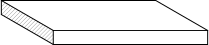
\includegraphics[scale=0.7]{\imgpath/measurement/piezo/piezo_plate_side}
        }}% c
    \sbox3{\subcaptionbox{Lateral stress, lateral particle displacement\label{sfig:piezo_radial_long}}{%
        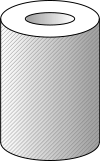
\includegraphics[scale=0.7]{\imgpath/measurement/piezo/piezo_radial_long}
        }}% d
    \sbox4{\subcaptionbox{Radial particle displacement\label{sfig:piezo_radial_flat}}{%
        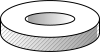
\includegraphics[scale=0.7]{\imgpath/measurement/piezo/piezo_radial_flat}
        }}% e
    \sbox5{\subcaptionbox{Radial particle displacement\label{sfig:piezo_axial_hole_flat}}{%
        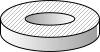
\includegraphics[scale=0.7]{\imgpath/measurement/piezo/piezo_axial_hole_flat}
        }}% f
    \sbox6{\subcaptionbox{Vertical stress, radial particle displacement\label{sfig:piezo_sphere}}{%
        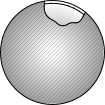
\includegraphics[scale=0.7]{\imgpath/measurement/piezo/piezo_sphere}
        }}% g
    \sbox7{\subcaptionbox{Radial particle displacement\label{sfig:piezo_axial_flat}}{%
        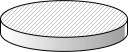
\includegraphics[scale=0.7]{\imgpath/measurement/piezo/piezo_axial_flat}
       }}% h
    \sbox8{\subcaptionbox{Radial particle displacement\label{sfig:piezo_radial_rod}}{%
        
\includegraphics[scale=0.7]{\imgpath/measurement/piezo/piezo_radial_rod}
       }}% i
    \centering
    {%
        \renewcommand{\arraystretch}{4}%
        \setlength{\tabcolsep}{2em}
        \begin{tabular}{ccc}
            \usebox0 & \usebox3 & \usebox6 \\
            \usebox1 & \usebox4 & \usebox7 \\
            \usebox2 & \usebox5 & \usebox8
        \end{tabular}
    }
    \caption[Piezoelectric designs]{Piezoelectric designs, where electrodes are placed on the shaded areas}
    \label{fig:piezo_designs}
\end{figure}

\begin{figure}[!htb]
    \centering
    \includestandalone[scale=1]{\imgpath/electronics/ic_flowchart/ic_flowchart}
    \caption[IC packages flowchart]{Flowchart of IC packages \cite{Tietze2008EC}}
    \label{fig:ic_flowchart}
\end{figure}

\begin{figure}[!htb]
    \centering
    \includestandalone[width=0.8\linewidth]{\imgpath/results/HAp024_TDat_x}
    \caption[Andromeda Measurement HAp024, Time Domain in X-Axis]{Measurement HAp024 in the time domain, excitation at point A, as shown in \figref{fig:andromeda_positions}}
    \label{fig:HAp024_TDat_x}
\end{figure}
\begin{figure}[!htb]
    \centering
    \includestandalone[width=0.8\linewidth]{\imgpath/results/HAp024_FFTa_x}
    \caption[Andromeda Measurement HAp024, FFT in X-Axis]{Measurement FFT HAp024, excitation at point A, as shown in \figref{fig:andromeda_positions}}
    \label{fig:HAp024_FFTa_x}
\end{figure}

\begin{figure}[!htb]
    \centering
    \includestandalone[width=0.8\linewidth]{\imgpath/results/HAp024_TDat_y}
    \caption[Andromeda Measurement HAp024, Time Domain in Y-Axis]{Measurement HAp024 in the time domain, excitation at point A, as shown in \figref{fig:andromeda_positions}}
    \label{fig:HAp024_TDat_y}
\end{figure}
\begin{figure}[!htb]
    \centering
    \includestandalone[width=0.8\linewidth]{\imgpath/results/HAp024_FFTa_y}
    \caption[Andromeda Measurement HAp024, FFT in Y-Axis]{Measurement FFT HAp024, excitation at point A, as shown in \figref{fig:andromeda_positions}}
    \label{fig:HAp024_FFTa_y}
\end{figure}
% ---- END MAIN PART ----

%bibliography:
\clearpage
\renewcommand*{\chapterpagestyle}{empty}
%\renewcommand*{\chapterheadstartvskip}{\vspace*{50pt}} % added to keep lyout after 25.08.15 (see studchapter.tex)
%\nocite{*}

\bibliography{references}
\addcontentsline{toc}{chapter}{Bibliography}


\end{document}
